\documentclass{beamer}

\usepackage{amsmath, amssymb}
\usepackage{tikz-cd}
\usepackage{xcolor}
\usepackage{graphicx}

\title{MAT414 - Modern Algebra - Permutation Groups}
\subtitle{Cycle Notation \cite{JAG2017}}
\author{\textbf{Miraj Samarakkody}}
\institute{Tougaloo College}
\date{Updated - \today}

\begin{document}

\begin{frame}
    \titlepage
\end{frame}




\begin{frame}
    \frametitle{Cycle Notation}

    Write the followings in the cyclic notations:
    \[
    \alpha = \begin{bmatrix}
        1 & 2 & 3& 4 & 5 & 6\\
        2& 1& 4 & 6 & 5 & 3
    \end{bmatrix}\quad \beta =  \begin{bmatrix}
        1 & 2 & 3& 4 & 5 & 6\\
        5& 3& 1 & 6 & 2 & 4
    \end{bmatrix}
    \] \pause
    Find \(\alpha \beta\). 

\end{frame}

\begin{frame}
    \frametitle{Properties of Permutations}

    \begin{block}{Theorem 5.1 - Products of Disjoint Cycles}
        Every permutation of a finite set can be written as a cycle or as a product of disjoint cycles. 
    \end{block}

\end{frame}

\begin{frame}
    \frametitle{Theorem 5.2}

    \begin{block}{Disjoint Cycles Commute}
        If the pair of cycles \(\alpha = (a_1,a_2, \dots, a_m)\) and \(\beta =(b_1, b_2, \dots, b_n)\) have no entries in common, then \(\alpha \beta = \beta \alpha\).
    \end{block}

\end{frame}

\begin{frame}
    \frametitle{Theorem 5.3}

    \begin{block}{Order of a Permutation}
        The order of a permutation of a finite set written in disjoint cycle form is the least common multiple of the lengths of the cycles. 
    \end{block}\pause

\vspace{0.2in}
    Find \begin{itemize}
        \item \(|(132)(45)|\)
        \item \(|(1432)(56)|\)
        \item \(|(123)(456)(78)|\)
        \item \(|(123)(145)|\)
    \end{itemize}

\end{frame}

\begin{frame}
    \frametitle{Example 5}

    Determine the orders of the elements of \(S_7\). 

\end{frame}

\begin{frame}
    \frametitle{Example 6}

    Determine the number of elements in \(S_7\) of order 12. 

\end{frame}

\begin{frame}
    \frametitle{Example 7}

    Determine the number of elements in \(S_7\) of order \(3\). 

\end{frame}

\begin{frame}
    \frametitle{Theorem 5.4}
    \begin{block}{Product of 2-Cycles}
          Every permutation of in \(S_n\), \(n>1\), is a product of \(2-\)cycles.   
    \end{block}

    

\end{frame}

\begin{frame}
    \frametitle{Example }

    \begin{align*}
        (1~2~3~4~5)=\\
        (1~6~3~2)(4~5~7)=
    \end{align*}

\end{frame}

\begin{frame}
    \frametitle{}
\begin{block}{Lemma}
    In \(S_n\), if \(\epsilon = \beta_1\beta_2 \beta_3 \dots \beta_r\), where the \(\beta_i\)'s are 2-cycles, then \(r\) is even. 
\end{block}
    

\end{frame}

\begin{frame}
    \frametitle{Theorem 5.5}

    \begin{block}{Always Even or Always Odd}
        If a permutation \(\alpha\) can be expressed as a product of an even (odd) number of 2-cycles, then every decomposition of \(\alpha\) into a product of \(2-\)cycles must have an an even (odd) number of \(2-\)cycles. \\
        \vspace{0.2in}
        In symbols, if \[\alpha = \beta_1 \beta_2 \dots \beta_r \text{ and } \alpha = \gamma_1 \gamma_2 \dots \gamma_s,\] where the \(\beta\)'s and \(\gamma\)'s are \(2-\)cycles, then \(r\) and \(s\) are both even or both odd.
    \end{block}

\end{frame}

\begin{frame}
    \frametitle{Even and Odd Permutations}
    \begin{block}{Definition}
        A permutation that can be expressed as a product of an even number of \(2-\)cycles is called an \textbf{even permutation}. A permutation that can be expressed as a product of an odd number of \(2-\)cycles is called an \textbf{odd permutation}.
    \end{block}
    

\end{frame}

\begin{frame}
    \frametitle{Even Permutations Form a Group} 
    \begin{block}{Theorem 5.6}
        The set of all even permutations of \(S_n\) is a subgroup of \(S_n\) and is denoted by \(A_n\).
    \end{block}
    

\end{frame}

\begin{frame}
    \frametitle{Alternating Group of Degree \(n\)}

    \begin{block}{Definition}
        The alternating group of degree \(n\), denoted \(A_n\), is the set of all even permutations of \(S_n\).
        
    \end{block}

\end{frame}

\begin{frame}
    \frametitle{Theorem}

    \begin{block}{Theorem 5.7}
        For \(n >1\), \(A_n\) has order \(n!/2\). 
    \end{block}

\end{frame}

\begin{frame}
    \frametitle{Example 10 - Rotations of a Tetrahedron}

    The 12 rotations of a regular tetrahedron can be conveniently described with the elements of \(A_4\). 
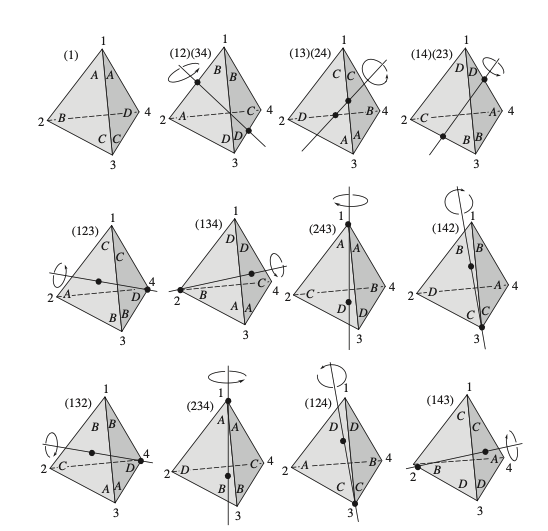
\includegraphics[scale=0.35]{Figures/fig_2.png}



\end{frame}

\begin{frame}
    \frametitle{Example 10 - Rotations of a Tetrahedron}

    The 12 rotations of a regular tetrahedron can be conveniently described with the elements of \(A_4\). 
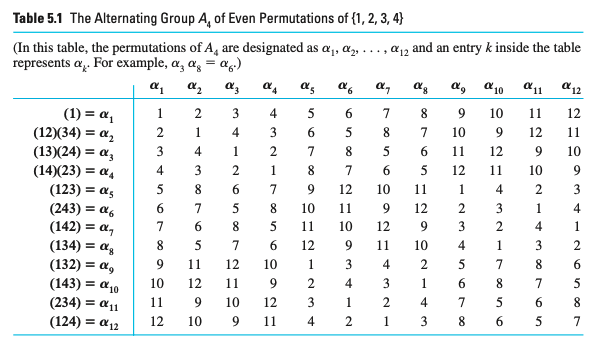
\includegraphics[scale=0.5]{Figures/fig_3.png}



\end{frame}

\begin{frame}
    \frametitle{Applications}

    Many molecules with chemical formulas of the form \(AB_4\), such as methane \((CH_4)\) and carbon tetrachloride \((CCl_4)\), have \(A_4\) as thier symmetry group. 

    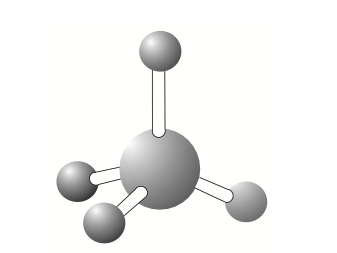
\includegraphics[scale=0.5]{Figures/fig_4.png}

\end{frame}

\begin{frame}
    \frametitle{Encryption Using a Permutation}

    \begin{itemize}
        \item An intersting application of permutations is in the field of cryptography.\pause
        \item cryptography is the science of encoding and decoding messages. \pause
        \item The process of encoding a message is called encryption, and the process of decoding a message is called decryption. \pause
        \item First known cryptosystme is th Caesar cipher. \pause
        \item The Caesar cipher is a substitution cipher, which means that each letter in the plaintext is replaced by a letter some fixed number of positions down the alphabet. 
    \end{itemize}

\end{frame}

\begin{frame}
    \frametitle{Rubik's Cube}

    \begin{itemize}
        \item It was invented in 1974 by Hungarian architect and professor of architecture Ernő Rubik. \pause
        \item The cube has 6 faces, each with 9 stickers of one of 6 solid colors. \pause
        \item The cube can be rotated about its axes, and the goal is to return the cube to its original state after it has been scrambled. \pause
        \item The cube has \(43,252,003,274,489,856,000\) possible configurations. \pause
        \item God’s number is 20, which means that any configuration of the cube can be solved in 20 moves or less.
    \end{itemize}

\end{frame}

\begin{frame}
    \frametitle{Rubick's Cube}

    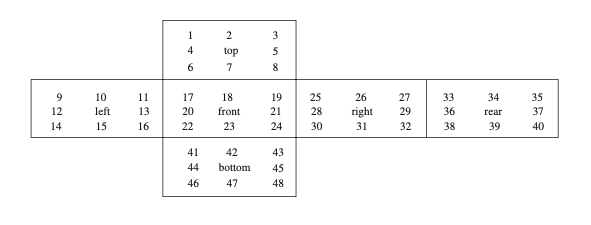
\includegraphics[scale=0.5]{Figures/fig_5.png}

\end{frame}





\begin{frame}
    \frametitle{References}
    \bibliographystyle{plain} % or another style like unsrt, alpha, etc.
    \bibliography{reference}  % omit the .bib extension
\end{frame}

\end{document}